Embedded system development processes are often presented on a ``V-diagram'', such as that shown in Fig. \ref{fig:vdiagram}. On this particular version of the diagram we show software development on one branch, hardware development on the other, and integration in the middle. While building tools to support familiar development processes, we also aim to improve the processes by shortening the length of design, development, and verification cycles.  This is achieved through model-based automation of development steps as well as providing feedback to earlier development stages as analysis results become available.  Our model-based prototyping toolchain models the software architecture (SwA), component design (CD), hardware architecture (HwA), system architecture (SY), and deployment (DPL) stages depicted in the diagram. The design of the modeling language and the toolchain capabilities are described more fully in ~\cite{aces08}.  

\begin{figure}[ht]
\centering
\includegraphics[width=\columnwidth]{figures/dev_diagram.jpg}
    \caption{Development flow for model-based embedded systems design tools}
    \label{fig:vdiagram}
\end{figure}

The development and prototyping process begins with (1) control design (in our case, using Simulink), where the controllers are modeled as hierarchical dataflow networks of function blocks ('subsystems' in Simulink terminology). Next, the subsystem models are elaborated to construct software component models (2), from which a software architecture model is built (3). The hardware platform models (4) describe the hardware architecture, including processors and buses. The software components ('tasks') and component interactions ('messages') are mapped to hardware elements in the deployment model (5). At this point, the suite of models could be subjected to schedulability analysis (6), followed by scheduling (7), and executable code is generated (8) from the functional blocks and the architecture models. The models are also rich enough to perform timing analysis using verification tools (like ~\cite{TrueTime}) The development process can take advantage of a hardware-in-the-loop simulator that is connected to the actually controller hardware. The simulator runs a high-fidelity, real-time dynamic simulation of the controlled 'plant' (a vehicle in our case). 

\begin{figure}[ht]
  \centering
  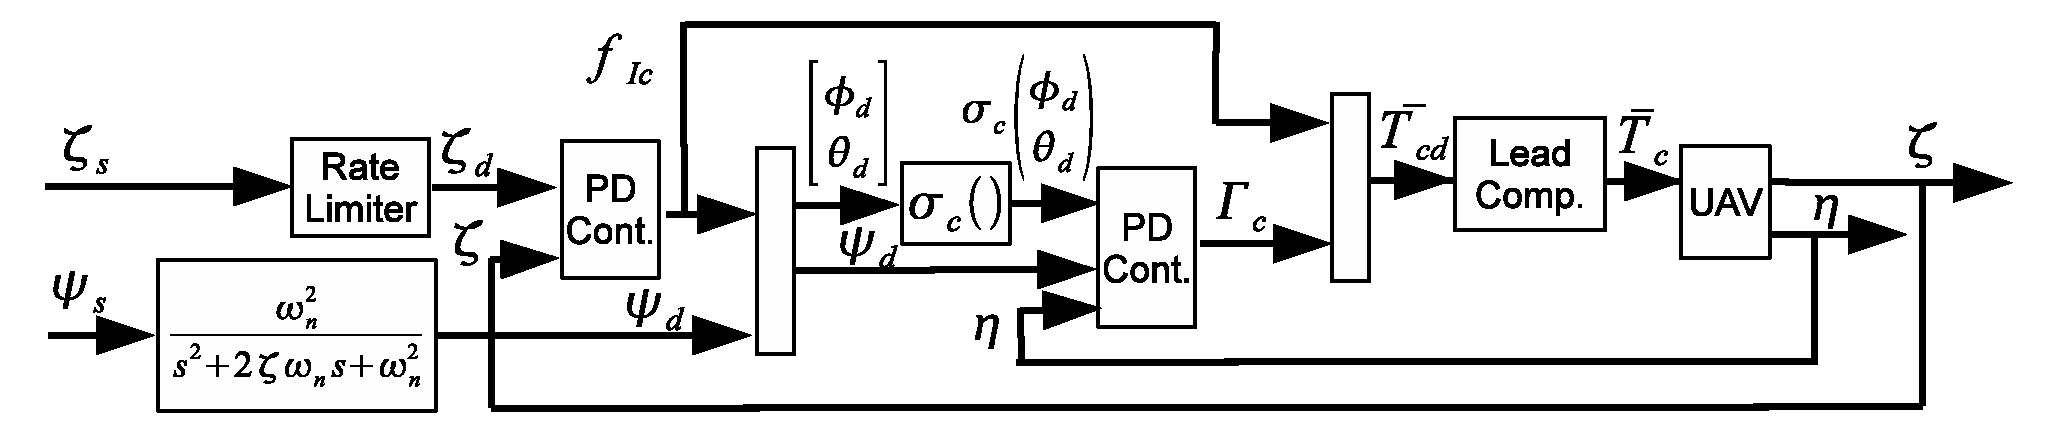
\includegraphics[width=\columnwidth]{figures/high_level_quad_control_sys}
  \caption{High-level quad-rotor control system diagram \cite{NJ:ISIS-08-911}}
  \label{fig:high_level_quad_control_sys}
\end{figure}

\SubSection{Passivity based control design and conic system verification}

Fig.~\ref{fig:high_level_quad_control_sys} depicts the nested control system used to explicitly control the quad-rotor's inertial position $\zeta$ and yaw $\psi$.  The inner control-loop for attitude $\eta = [\phi,\theta,\psi]^\mathtt{T}$ consists of a passive proportional-derivative (PD) controller.  The outer control-loop for $\zeta$ is also a PD controller.  A non-linear mapping based on the system kinematics, desired inertial control force $f_{Ic}$ and desired yaw $\psi_d$ results in a corresponding desired roll $\phi_d$ and pitch $\theta_d$ which were correspondingly limited to the range $[-\frac{\pi}{4},\frac{\pi}{4}]$.  The desired yaw, and range limited roll and pitch depicted respectively as $\psi_d$ and $\sigma_c([\phi_d,\theta_d]^\mathtt{T})$ are inputs to the attitude PD controller in which $\Gamma_c$ is the desired control torque.  However, neither the desired control torque $\Gamma_c$ nor the inertial control force $f_{Ic}$ can be explicitly applied to the quad-rotor aircraft.  Instead, a matrix transformation is used to determine the desired rotor control thrust $\bar{T}_{cd}$.  Finally, in order to compensate for the slow rotor dynamics a passive lead compensator is implemented to determine the corresponding rotor thrust command $\bar{T}_c$ which is sent to the corresponding four rotors on the quad-rotor aircraft (denoted UAV) in the figure.  For additional details the interested reader is referred to \cite{NJ:ISIS-08-911}.

\begin{figure}[ht]
\centering
%\includegraphics[width=\columnwidth]{figures/inertial_control.jpg}
%\includegraphics[width=\columnwidth]{figures/starmac_inertial.pdf}
\includegraphics[width=\columnwidth]{figures/starmac_inertial_controller.png}
    \caption{Simulink model for the nonlinear inertial controller}
    \label{fig:controller}
\end{figure}

Simulink was used to design, test, and verify our controller, including the inertial-control subsystem depicted in Fig.~\ref{fig:controller}.  Simulink's block-based graphical design paradigm is very expressive and intuitive to control designers.  However, nonlinearity and model complexity (i.e., the high degree of interconnection between components) can make such designs difficult to analyze. On the other hand, such safety-critical control systems are examples of the \emph{high-confidence design} paradigm. Aircraft certification authorities require proof (or at least evidence) that controllers, software designs, and implementations meet safety requirements \cite{DO178B}.  Automated verification can be intractable for large designs, so we prefer methods which facilitate \emph{design decoupling}.  Decoupling means that component-level analysis together with adherence to composition rules are sufficient to ensure correct behavior. Here we use passivity based controller design techniques \cite{NJ:ISIS-08-911} to facilitate decoupling. 

Passivity is a good example of a property which facilitates design decoupling.  In control theory, passive systems do not introduce new energy into the overall system.  Furthermore, systems which consist of cascades of two passive systems can be composed using a nested feed-back structure which results in a stable configuration --- in fact, most PD controllers for non-linear passive systems depend on this property \cite{NJ:ISIS-08-911}.  Verifying stability of a network of passive components requires analysis of each component at the local level, with extended joint state space analysis of components connected serially.  A simple topology check is all that is required beyond this.  Passivity may be verified locally for linear components using linear matrix inequalities (LMIs), where a convex optimization problem and associated solver determine whether certain matrix conditions hold.  We are investigating methods to verify sector conditions (for which passivity is a special case) related to stability for both linear and nonlinear systems \cite{NJ:ISIS-08-911}. Our prototyping tools must handle a wide range of designs, including nonlinear designs and complex networks of components.  One reason for choosing the Starmac example was to demonstrate our capabilities with nonlinear models.

\SubSection{Model-Based Design}

Model-based design is performed with the help of design languages that are often graphical. For our environment we have developed a domain-specific modeling language (DSML), ESMoL, that is specified by metamodels using the Generic Modeling Environment\cite{karsai:mic}.  A DSML metamodel restricts design models to structurally correct ones, eliminating large classes of potential errors from a design.  Structural correctness is not sufficient by itself; the DSML must have well-defined behavioral semantics to complete the definition.  For example, Simulink allows a designer to construct models from libraries of functional blocks.  Any properly constructed model can then be simulated to assess the design, so Simulink has a complete behavioral semantics that is defined by the simulation engine.  Note that behavior validated in simulation may change dramatically once the various functions are implemented and deployed on a platform, so additional modeling is required to capture platform effects in control designs. metamodels using the Generic Modeling Environment\cite{karsai:mic}.  A DSML metamodel restricts design models to structurally correct ones, eliminating large classes of potential errors from a design.  Structural correctness is not sufficient by itself; the DSML must have well-defined behavioral semantics to complete the definition.  For example, Simulink allows a designer to construct models from libraries of functional blocks.  Any properly constructed model can then be simulated to assess the design, so Simulink has a complete behavioral semantics that is defined by the simulation engine.  Note that behavior validated in simulation may change dramatically once the various functions are implemented and deployed on a platform, so additional modeling is required to capture platform effects in control designs.

\begin{figure}[ht]
\centering
%\includegraphics[width=\columnwidth]{figures/inertial_control_gme.jpg}
\includegraphics[width=\columnwidth]{figures/starmac_gme.png}
    \caption{ESMoL model for the inertial controller (imported from Simulink)}
    \label{fig:gme_ctrl}
\end{figure}

Models in ESMoL\cite{aces08} describe distributed embedded control systems subject to time-triggered execution semantics.  The time-triggered architecture (TTA) follows a distributed, timed model of computation in which all tasks and message transfers between tasks execute periodically, at pre-calculated time instants\cite{kopetz:2001-22a}. The clocks of computing nodes in the system are tightly synchronized. This technique enables distributed fault-tolerance techniques such as detecting and isolating faulty nodes, and deterministic execution of replicated computations.  Each task has logical execution time semantics\cite{henzinger01giotto}, which means that all input messages are available before a task consuming them is released, and output messages of the task are sent at precisely defined points in time, after the task has finished.  Any task requiring data can not start before the deadline of the sending task plus the transfer time of the message.  Any well-formed ESMoL model has a corresponding time-triggered model of execution whose global behavior may be assessed at design-time, by schedule determination.

ESMoL is a design language that includes the discrete-time subset of Simulink and Stateflow as sub-modeling languages, but it extends those with modeling constructs for componentization, platform modeling, and deployment modeling. It provides an end-to-end approach for connecting the controller models to actual implementation and deployment, where the design engineer has a large freedom in making choices the influence the physical realization of controllers, and has the opportunity to perform various analysis steps in the process.

%\subsubsection*{Import and Architecture model}

\begin{figure}[ht]
\centering
\includegraphics[height=1in]{figures/sw_arch.jpg}
    \caption{ESMoL model for the software component architecture}
    \label{fig:sw_arch}
\end{figure}

\textbf{Import and Architecture Model.} First, the designer imports a Simulink model into the ESMoL modeling tool (built using GME).  Fig. \ref{fig:gme_ctrl} shows an example --- the inertial controller.  The imported dataflow model is a structural replica of the original, though the time-triggered semantics of ESMoL allows use of only Simulink blocks and structures that execute periodically, following a 'clocked-synchronous' model. Subsystems in the GME replica are used to create the components for a software architecture model, as in Fig. \ref{fig:sw_arch}.  Generally, the architecture mimics the structure of the Simulink functional design, possibly with multiple functional block instances or external code fragments added to the component fabric.  Blocks in this diagram correspond to imperative (C) code that will implement the specified functions.  Connections represent either direct synchronous procedure calls between components, or time-triggered messages delivered by the network.

%\subsubsection*{Platform model}

\begin{figure}[ht]
\centering
\includegraphics[height=1in]{figures/platform.jpg}
    \caption{ESMoL model for the computational hardware (Gumstix/Robostix pair)}
    \label{fig:platform}
\end{figure}

\textbf{Platform Model.} In our experimental setup, the hardware for the Starmac control system consists of a Gumstix Verdex embedded processing module, with a Robostix I/O expansion board.  The Gumstix is a PXA-based processing board with both wired and wireless Ethernet as well as expansion connectors.  The Robostix has an Atmega 128 microcontroller with numerous ports for collecting sensor data or providing actuation signals.  One Robostix UART is dedicated to the 'plant' data connection (see below).  An I2C bus links the Gumstix with the Robostix, which exchange sensor, state, and control data.  The ESMoL model of the platform is appropriately simple (Fig. \ref{fig:platform}).

The time-triggered platform is realized in a simple, portable software implementation of the TTA\cite{RT_Thesis}.  The FRODO virtual machine (VM) implements the time-triggered execution of  tasks, and has a communications layer which handles the buffering and timed transfers of data messages.  The current version runs on generic Linux (on the Gumstix) as well as the FreeRTOS (on the AVR).  If a new processor or OS is used, the VM needs to be ported to that new platform. 

%\subsubsection*{Deployment model}

\begin{figure}[ht]
\centering
\includegraphics[width=\columnwidth]{figures/deploy.jpg}
    \caption{ESMoL model for task deployment (center): the outer loop task (top) sends trajectory information to the inner loop task (bottom), which handles sensor data and controls attitude.}
    \label{fig:deploy}
\end{figure}

\textbf{Deployment Model.} The deployment model contains tasks and messages, which connect the software and hardware elements.  Tasks encapsulate software components that execute at the same periodic rate, and assign them to a processing node.  The software components within a task are specified via references ('pointers') to component instances in the software architecture model.  Messages implement the time-triggered communications defined as connections in the software architecture.  Message references connecting tasks ensure that the sender and receiver point to the same message object.  Fig. \ref{fig:deploy} shows the details of the deployment model for our example.

%\subsubsection*{Schedule Computation}

\textbf{Schedule Computation.} Schedule determination is one type of analysis that has been integrated into our rapid development environment.  Fig. \ref{fig:roundtrip} depicts the round-trip scheduling process. A model transformation generates a configuration file for the scheduling tool.  Once run, the scheduling tool internally converts the configuration to finite-domain integer constraint models\cite{offlinescheduling} which are then solved using the Gecode constraint solver tool\cite{gecode}.  If a schedule can be found, then the result is written back into the design model using modeling tool's API.  The running example is trivial --- each processor has only a single task and one message receiver (the other end).  Both tasks execute at the same time, and data transfers can occur immediately after each task deadline on the full-duplex serial link.  Each task invocation gets its data (previously transferred by the virtual machine) from a buffer.

To validate the controller performance with respect to the computed schedule, we use the TrueTime \cite{TrueTime} blocks in Simulink to perform platform-specific resimulation.  TrueTime provides a framework for modeling platforms (processors, networks, scheduling, and protocols), and for exploring the effects of the platform (delays, quantization effects). 

\begin{figure}[ht]
\centering
\includegraphics[width=\columnwidth]{figures/roundtrip.jpg}
    \caption{Integration of the scheduling tool with the modeling environment}
    \label{fig:roundtrip}
\end{figure}

\SubSection{Software synthesis}

Software synthesis creates executable code from well-formed models.  In our tools, code generation occurs at two points: the platform-independent code dealing with the actual (control) functions in the design, and platform-dependent 'glue' code specific to the actual software platform and the chosen model of computation.  This latter includes configuration code, and task wrappers for functional code. For functional code generation we use a graph transformation-based technique \cite{KS:ISIS-04-505}. For platform-specific code we use a simple, template-based code generator that relies on the model access API-s provided by the modeling environment. This generator produces code for task wrappers, message structures, timing information (provided by the scheduler), and configuration. The complete execution environment for the target platform consists all of the generated code, the virtual machine code, and the platform operating system. 